\documentclass{standalone}
\usepackage{tikz}
\usetikzlibrary{arrows.meta,decorations.pathmorphing}
\usepackage{amsmath}

\usepackage[T1]{fontenc}
\usepackage{newtxtext}
\usepackage{newtxmath}

% neutral: in figure 20 colour is the gap width, and the sketch is generic;
% the line styles of the disturbances are those of L2POvsX*.pdf
\colorlet{pdark}{black!85}
\colorlet{pmid}{black!55}

\newcommand{\fsize}{\fontsize{8.7}{10.44}\selectfont}

%% ── geometry of the sketch (arbitrary units) ─────────────────────────────
\def\xg{0.3}    % upstream gap edge
\def\xe{1.8}    % downstream gap edge, where the 3D disturbances start growing
\def\xr{10.6}   % right end of the plot
\def\sl{0.6}    % slope sigma of the 3D disturbances (log amplitude per unit x)
\def\yb{4.7}    % breakdown level
\def\ys{5.3}    % saturation level
\def\ytop{5.9}  % top of the amplitude axis
\def\yw{6.9}    % wall in the flow sketch
%% seed levels of the 3D disturbances, one label height apart at least
\def\yA{3.2}    % A = 1e-3
\def\yB{1.9}    % A = 1e-5
\def\yC{0.3}    % A = machine epsilon (round-off)
\pgfmathsetmacro{\xbA}{\xe+(\yb-\yA)/\sl}
\pgfmathsetmacro{\xbB}{\xe+(\yb-\yB)/\sl}
\pgfmathsetmacro{\xbC}{\xe+(\yb-\yC)/\sl}

% seed level upstream, exponential growth from the gap edge, then saturation
\newcommand{\disturbance}[3]{% style, seed level, breakdown position
	\draw[pdark, #1] (0,#2) -- (\xe,#2) -- (#3,\yb)
	.. controls ({#3+0.45},{\yb+0.45*\sl}) and ({#3+0.5},\ys) .. ({#3+1.1},\ys)
	-- (\xr,\ys);
}
% label on top of a horizontal level, at the left of the plot
\newcommand{\levellabel}[2]{\node[pdark, above right, inner sep=1.5pt] at (0.05,#1) {#2};}

\begin{document}
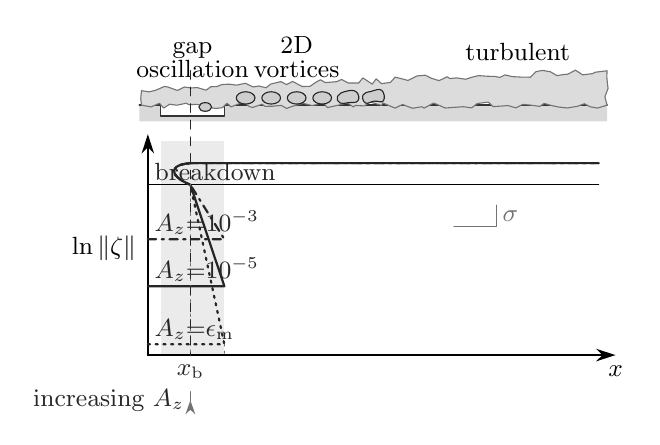
\begin{tikzpicture}[x=0.54cm, y=0.46cm, font=\fsize, line cap=round, line join=round]

	%% ── amplitude plot ──────────────────────────────────────────────────────
	\fill[black!8] (\xg,0) rectangle (\xe,\ytop);

	\draw[thick, -{Stealth[length=7pt,width=4.5pt]}] (0,0) -- (\xr+0.4,0) node[below] {$x$};
	\draw[thick, -{Stealth[length=7pt,width=4.5pt]}] (0,0) -- (0,\ytop+0.2);
	\node[left] at (-0.05,{\ytop/2}) {$\ln\|\zeta\|$};

	% breakdown level
	\draw[black, thin] (0,\yb) -- (\xr,\yb);
	\levellabel{\yb}{breakdown}

	% three-dimensional disturbances for three levels of the forcing
	\disturbance{thick, dash dot}{\yA}{\xbA}
	\disturbance{thick}{\yB}{\xbB}
	\disturbance{thick, dotted}{\yC}{\xbC}
	\levellabel{\yA}{$A_z{=}10^{-3}$}
	\levellabel{\yB}{$A_z{=}10^{-5}$}
	\levellabel{\yC}{$A_z{=}\epsilon_\mathrm{m}$}

	% common start of the growth, at the downstream edge of the gap
	\draw[pmid, dotted, semithick] (\xe,\yC) -- (\xe,0);

	% growth rate, on the round-off curve
	\pgfmathsetmacro{\ya}{\yC+\sl*(7.2-\xe)}
	\pgfmathsetmacro{\yc}{\yC+\sl*(8.2-\xe)}
	\draw[pmid] (7.2,\ya) -- (8.2,\ya) -- (8.2,\yc);
	\node[pmid, right, inner sep=2pt] at (8.2,{(\ya+\yc)/2}) {$\sigma$};

	% breakdown positions
	\foreach \xb in {\xbA,\xbC}
	\draw[pmid, dotted, semithick] (\xb,\yb) -- (\xb,0);
	\draw[-{Stealth[length=5pt,width=3.5pt]}, pmid, semithick] (\xbC,-1.25) -- (\xbA,-1.25)
	node[left, pdark, inner sep=2pt] {increasing $A_z$};

	%% ── flow sketch, for A = 1e-5 ───────────────────────────────────────────
	\fill[black!15] (-0.2,\yw) -- (\xg,\yw) -- (\xg,\yw-0.3) -- (\xe,\yw-0.3) -- (\xe,\yw)
	-- (\xr+0.2,\yw) -- (\xr+0.2,\yw-0.45) -- (-0.2,\yw-0.45) -- cycle;
	\draw[black!80, semithick] (-0.2,\yw) -- (\xg,\yw) -- (\xg,\yw-0.3) -- (\xe,\yw-0.3) -- (\xe,\yw) -- (\xr+0.2,\yw);

	% turbulent boundary layer downstream of breakdown
	\pgfmathsetseed{7}
	\fill[pmid!25, draw=pmid, decorate, decoration={random steps, segment length=2.5pt, amplitude=1.2pt}]
	(\xbB-0.15,\yw) -- (\xbB-0.15,\yw+0.4) -- (\xr+0.2,\yw+0.95) -- (\xr+0.2,\yw) -- cycle;

	% train of two-dimensional vortices shed from the gap, the last ones distorted
	\draw[pdark, fill=pmid!35] (1.35,\yw-0.05) ellipse (0.15 and 0.12);
	\foreach \x in {2.3,2.9,3.5,4.1}
	\draw[pdark, fill=pmid!35] (\x,\yw+0.2) ellipse (0.22 and 0.17);
	\foreach \x/\d in {4.7/0.04, 5.3/0.08}
	\draw[pdark, fill=pmid!35] plot[smooth cycle, tension=0.8] coordinates {
		({\x-0.24},{\yw+0.2+\d}) ({\x-0.05},{\yw+0.38}) ({\x+0.2},{\yw+0.33+\d})
		({\x+0.24},{\yw+0.12}) ({\x+0.02},{\yw+0.03+\d}) ({\x-0.18},{\yw+0.06})};

	\node[above, align=center] at (1.05,\yw+0.5) {gap\\[-2pt]oscillation};
	\node[above, align=center] at (3.5,\yw+0.5) {2D\\[-2pt]vortices};
	\node[above] at (8.7,\yw+0.95) {turbulent};

	% link between the flow sketch and the amplitude plot
	\draw[pdark, dashed, semithick] (\xbB,\yw+0.95) -- (\xbB,0) node[below, pdark] {$x_\mathrm{b}$};
\end{tikzpicture}
\end{document}
